\chapter{Themenkorb - Relationales Datenbankmodell}

\section{DDL}
\subsection{Datentypen}
\begin{itemize}
    \item CHAR(n) $\implies$ Fixed-length, Rest wird mit Leerzeichen aufgefüllt bzw. abgeschnitten!
    \item VARCHAR(n) $\implies$ Variable Länge (max. n)
    \item Date
    \item Timestamp
    \item NUMBER(s, p) $\implies$ Einzige Zahlen-Datentyp in Oracle: s gibt die Gesamtstellen an, p die nach dem Komma
    \begin{itemize}
        \item NUMERIC, DECIMAL sind nur die ANSII Name für diese Datentypen!
        \item Float / Real / Double Precision steht in den Docs zwar als Subtyp von Number, wird aber (im Unterschied zu NUMERIC\dots) als FLOAT in Describe angezeigt!
    \end{itemize}
\end{itemize}

\subsection{Constraints}
\begin{itemize}
    \item NOT NULL $\implies$ Null-Werte sind nicht erlaubt
    \item UNIQUE $\implies$ Der Wert muss innerhalb der Spalte einzigartig sein
    \item PRIMARY KEY 
    \begin{itemize}
        \item Sofort nach dem Attribut, wenn er nur aus einem Attribut besteht
        \item Am Ende des Tables, wenn er aus mehreren Attributen besteht!
        \begin{figure}[H]
            \centering
            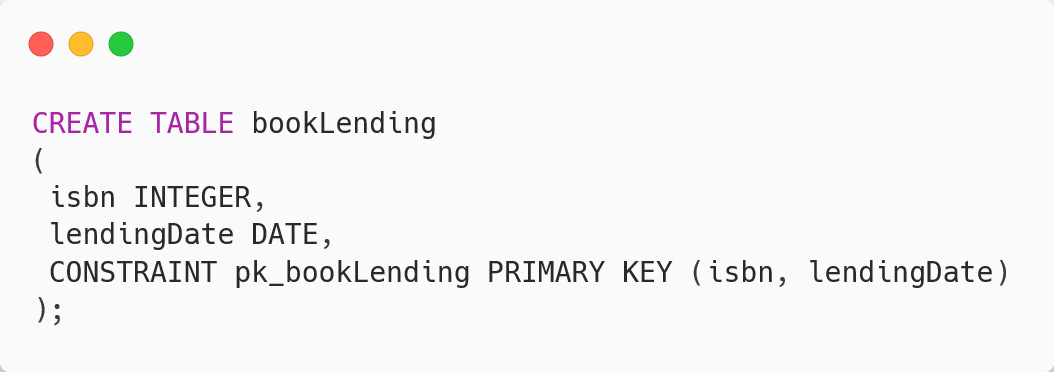
\includegraphics[scale=.3]{res/themenkorb_3/pk.png}
        \end{figure}
    \end{itemize}
    \item FOREIGN KEY
    \begin{itemize}
        \item Am Ende des Tables
        \begin{figure}[H]
            \centering
            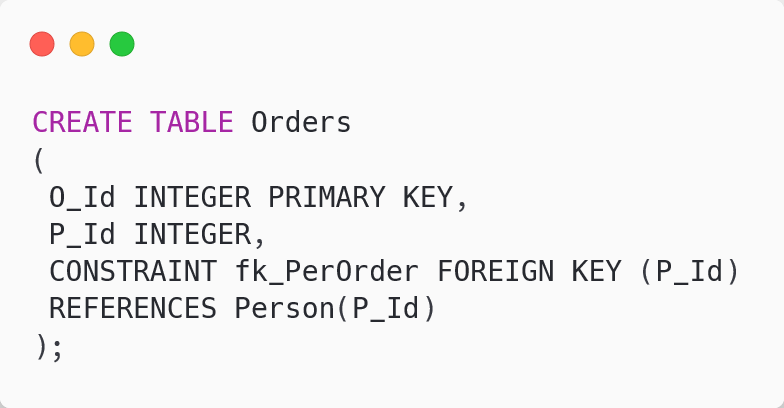
\includegraphics[scale=.3]{res/themenkorb_3/fk.png}
        \end{figure}
    \end{itemize}
    \item CHECK $\implies$ Um sicherzustellen, dass ein Wert ein gewisses Kriterium erfüllt
    \begin{figure}[H]
        \centering
        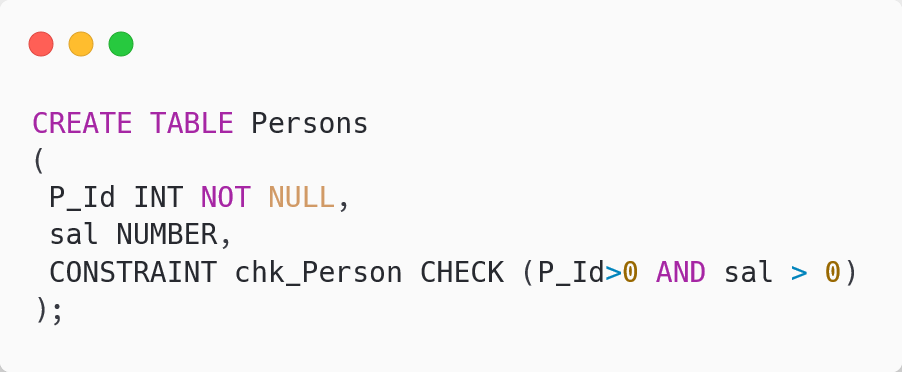
\includegraphics[scale=.3]{res/themenkorb_3/check.png}
    \end{figure}
    \item DEFAULT $\implies$ Default-Wert, falls dieser beim Insert weggelassen wird
\end{itemize}

\subsection{Tabellen im Nachinein bearbeiten}
\begin{itemize}
    \item Vor allem bei FKs relevant, da dann nicht mehr auf die Reihenfolge von Tabellen geachtet werden muss!
    \item Es können Constraints \& Spalten bearbeitet werden!
    \begin{itemize}
        \item Constraints
        \begin{figure}[H]
            \centering
            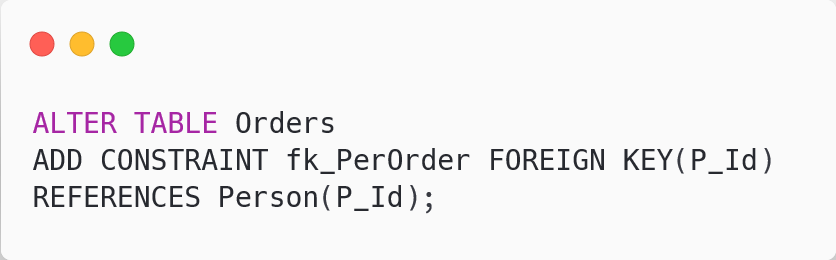
\includegraphics[scale=.3]{res/themenkorb_3/alter_constraint.png}
        \end{figure}
        \item Spalten
        \begin{figure}[H]
            \centering
            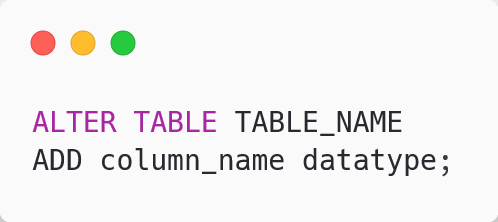
\includegraphics[scale=.3]{res/themenkorb_3/add_col.png}
        \end{figure}
        \begin{figure}[H]
            \centering
            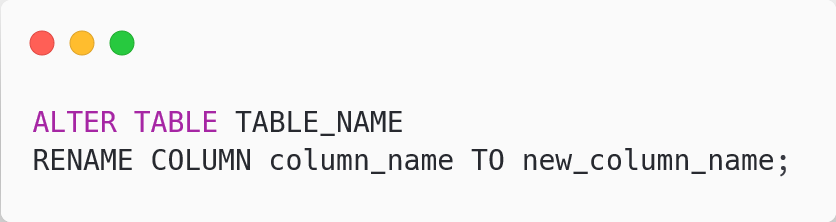
\includegraphics[scale=.3]{res/themenkorb_3/rename_col.png}
        \end{figure}
        \begin{figure}[H]
            \centering
            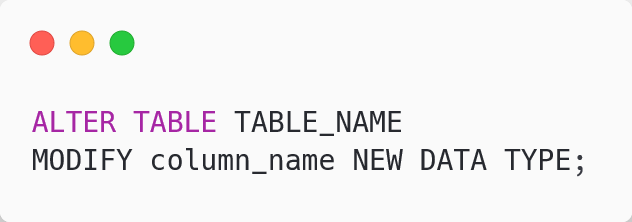
\includegraphics[scale=.3]{res/themenkorb_3/update_data_type.png}
        \end{figure}
    \end{itemize}
    \item Es können sowohl einzelne Constraints, als auch Columns und Tables gedroppt werden!
    \begin{itemize}
        \item Beim Droppen von Tables empfiehlt es sich, vorher die Foreign-Key-Constraints zu entfernen, damit im Falle von Cascade Constraints keine Daten aus Versehen gelöscht werden!
    \end{itemize}
\end{itemize}

\section{DML}
\subsection{Views}
\begin{itemize}
    \item Sind das Ergebnis eines Select-Statements
\end{itemize}

\subsection{Sequences}
\begin{itemize}
    \item Erstellen
    \item Beim Inserten --> sequence.NEXTVAL
    \begin{figure}[H]
        \centering
        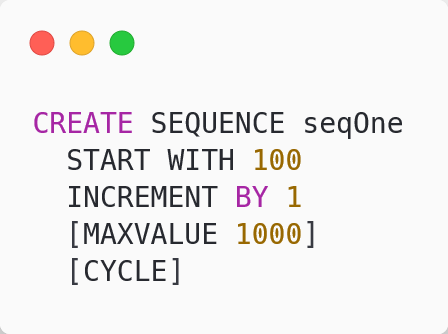
\includegraphics[scale=.3]{res/themenkorb_3/create_sequence.png}
    \end{figure}
\end{itemize}

\subsection{MERGE}
\begin{itemize}
    \item Inserted ein Item, falls das gesuchte nicht gefunden wurde
    \item Updated ein existierendes Item, falls es gefunden wurde
\end{itemize}

\section{Normalisierung}
\subsection{Normalformen}
\subsubsection{Nullte Normalform}
\begin{itemize}
    \item Mehrere Werte stehen in einer Zeile:
\end{itemize}
\begin{figure}[H]
    \centering
    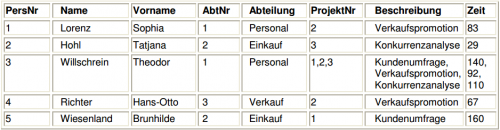
\includegraphics[width=\textwidth]{res/themenkorb_3/normalization_pic1.png}
\end{figure}
\subsubsection{Erste Normalform}
\begin{itemize}
    \item Jede Zeile enthält nur einen Wert
    \item Es muss ein Primary Key gefunden werden (\textbf{unterstreichen}!), welcher jede \textbf{Zeile} eindeutig kennzeichnet!
\end{itemize}
\begin{figure}[H]
    \centering
    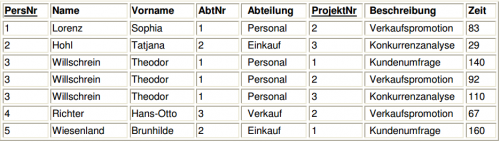
\includegraphics[width=\textwidth]{res/themenkorb_3/normalization_pic2.png}
\end{figure}
\subsubsection{Zweite Normalform}
\begin{itemize}
    \item Die Relation befindet sich in der 1. Normalform + jedes Attribut ist vom Gesamtschlüssel der Relation abhängig, und nicht nur von einem Teil!
    \item Praxis: Ursprüngliche Tabelle in mehrere unterteilen, sodass oben genannte Anforderungen erfüllt sind!
    \begin{itemize}
        \item Diese Tables dürfen nur Attribute enthalten, die vom gesammten PK abhängig sind $\implies$ Es kann sein, dass eine Relation 2 Primary Key Attribute benötigt!
    \end{itemize}
\end{itemize}
\begin{figure}[H]
    \centering
    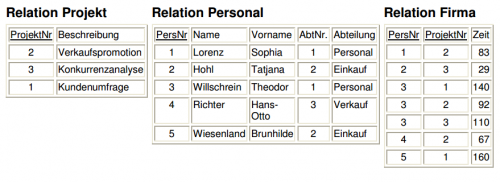
\includegraphics[width=\textwidth]{res/themenkorb_3/normalization_pic3.png}
\end{figure}
\subsubsection{Dritte Normalform}
\begin{itemize}
    \item Die Relation befindet sich in der 2. Normalform + Kein Attribut ist von einem anderen Nicht-Schlüssel-Attribut abhängig!
\end{itemize}
\begin{figure}[H]
    \centering
    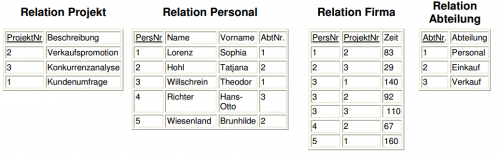
\includegraphics[width=\textwidth]{res/themenkorb_3/normalization_pic6.png}
\end{figure}

\subsection{Anwendung - Zirkelbezug}
\begin{itemize}
    \item Problem des Zirkelbezugs
    \begin{itemize}
        \item Eine Entity kann von einer Ausgangsentity auf 2 verschiedene Wege erreicht werden:
        \begin{figure}[H]
            \centering
            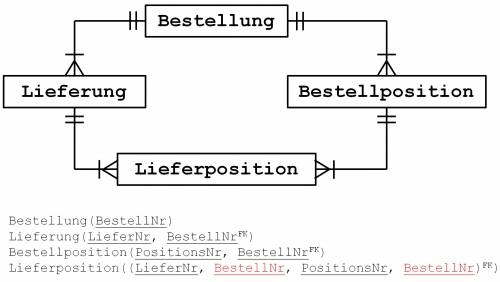
\includegraphics[scale=.8]{res/themenkorb_3/zirkelbezug_1.jpg}
        \end{figure}
        \item Je nachdem, ob über die Lieferung oder die Bestellposition auf die Bestellung zugegriffen wird, kann es zu unterschiedlichen Ergebnissen kommen!
    \end{itemize}
    \item Lösung: Die doppelten Attribute werden zu einem zusammengezogen und in einen Foreign Key verpackt:
    \begin{figure}[H]
        \centering
        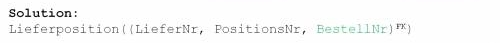
\includegraphics[scale=.8]{res/themenkorb_3/zirkelbezug_2.jpg}
    \end{figure}
\end{itemize}

\subsection{Abhängigkeitsdiagramm - Beispiele}
\subsubsection{2. Normalform}
\begin{figure}[H]
    \centering
    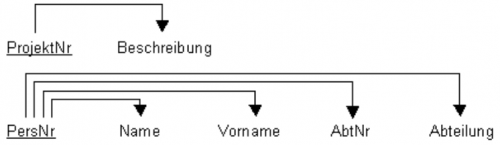
\includegraphics[width=\textwidth]{res/themenkorb_3/normalization_pic4.png}
\end{figure}
\subsubsection{3. Normalform}
\begin{figure}[H]
    \centering
    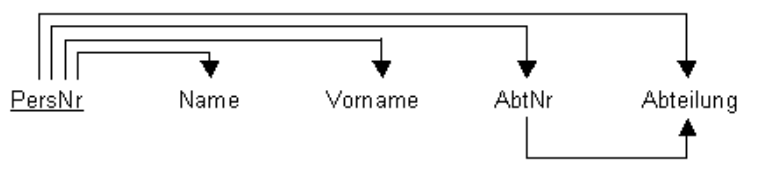
\includegraphics[width=\textwidth]{res/themenkorb_3/normalization_pic7.png}
\end{figure}